\documentclass[11pt]{article}
\usepackage[margin = 1in]{geometry}
\usepackage{amsmath}
\usepackage{amssymb}
\usepackage{amsthm}
\usepackage{graphicx}
\usepackage{enumitem}
\usepackage{url}
\usepackage[parfill]{parskip}
\usepackage{listings}
\newcommand{\skipline}{\vspace{\baselineskip}}
\newcommand{\spacer}{\noalign{\medskip}}
\newcommand{~}{\sim}
\newenvironment{problem}[1]{\textbf{Problem #1: }}{\newpage}
\usepackage{caption}
\usepackage{subcaption}
\usepackage[utf8]{inputenc}
\usepackage{xcolor}
\definecolor{codegreen}{rgb}{0,0.6,0}
\definecolor{codegray}{rgb}{0.5,0.5,0.5}
\definecolor{codepurple}{rgb}{0.58,0,0.82}
\definecolor{backcolour}{rgb}{0.95,0.95,0.92}
\lstdefinestyle{mystyle}{
	backgroundcolor=\color{backcolour},   
	commentstyle=\color{codegreen},
	keywordstyle=\color{magenta},
	numberstyle=\tiny\color{codegray},
	stringstyle=\color{codepurple},
	basicstyle=\ttfamily\footnotesize,
	breakatwhitespace=false,         
	breaklines=true,                 
	captionpos=b,                    
	keepspaces=true,                 
	numbers=left,                    
	numbersep=5pt,                  
	showspaces=false,                
	showstringspaces=false,
	showtabs=false,                  
	tabsize=2
}
\lstset{style=mystyle}
\newcommand{\qrarrow}{\quad \rightarrow \quad}
\newcommand{\qqrarrow}{\qquad \rightarrow \qquad}
\newcommand{\partiald}[2]{\frac{\partial #1}{\partial #2}}

\begin{document}
	
	\begin{center}
		\textbf{Worksheet 1} \\
		\textbf{Mechanics} \\
		\textbf{Physics 195} \\
		\textbf{Stephen Giang ID: 0005678772} \\
		\skipline \skipline
	\end{center}

	\begin{problem}{1}
		The diagrams below each show a vector in the $xy$-plane.  For each vector:  calculate the $x$-component and the $y$-component of the vector. Give your answers to 2 decimal places.
		\begin{figure}[h!]
			\centering
			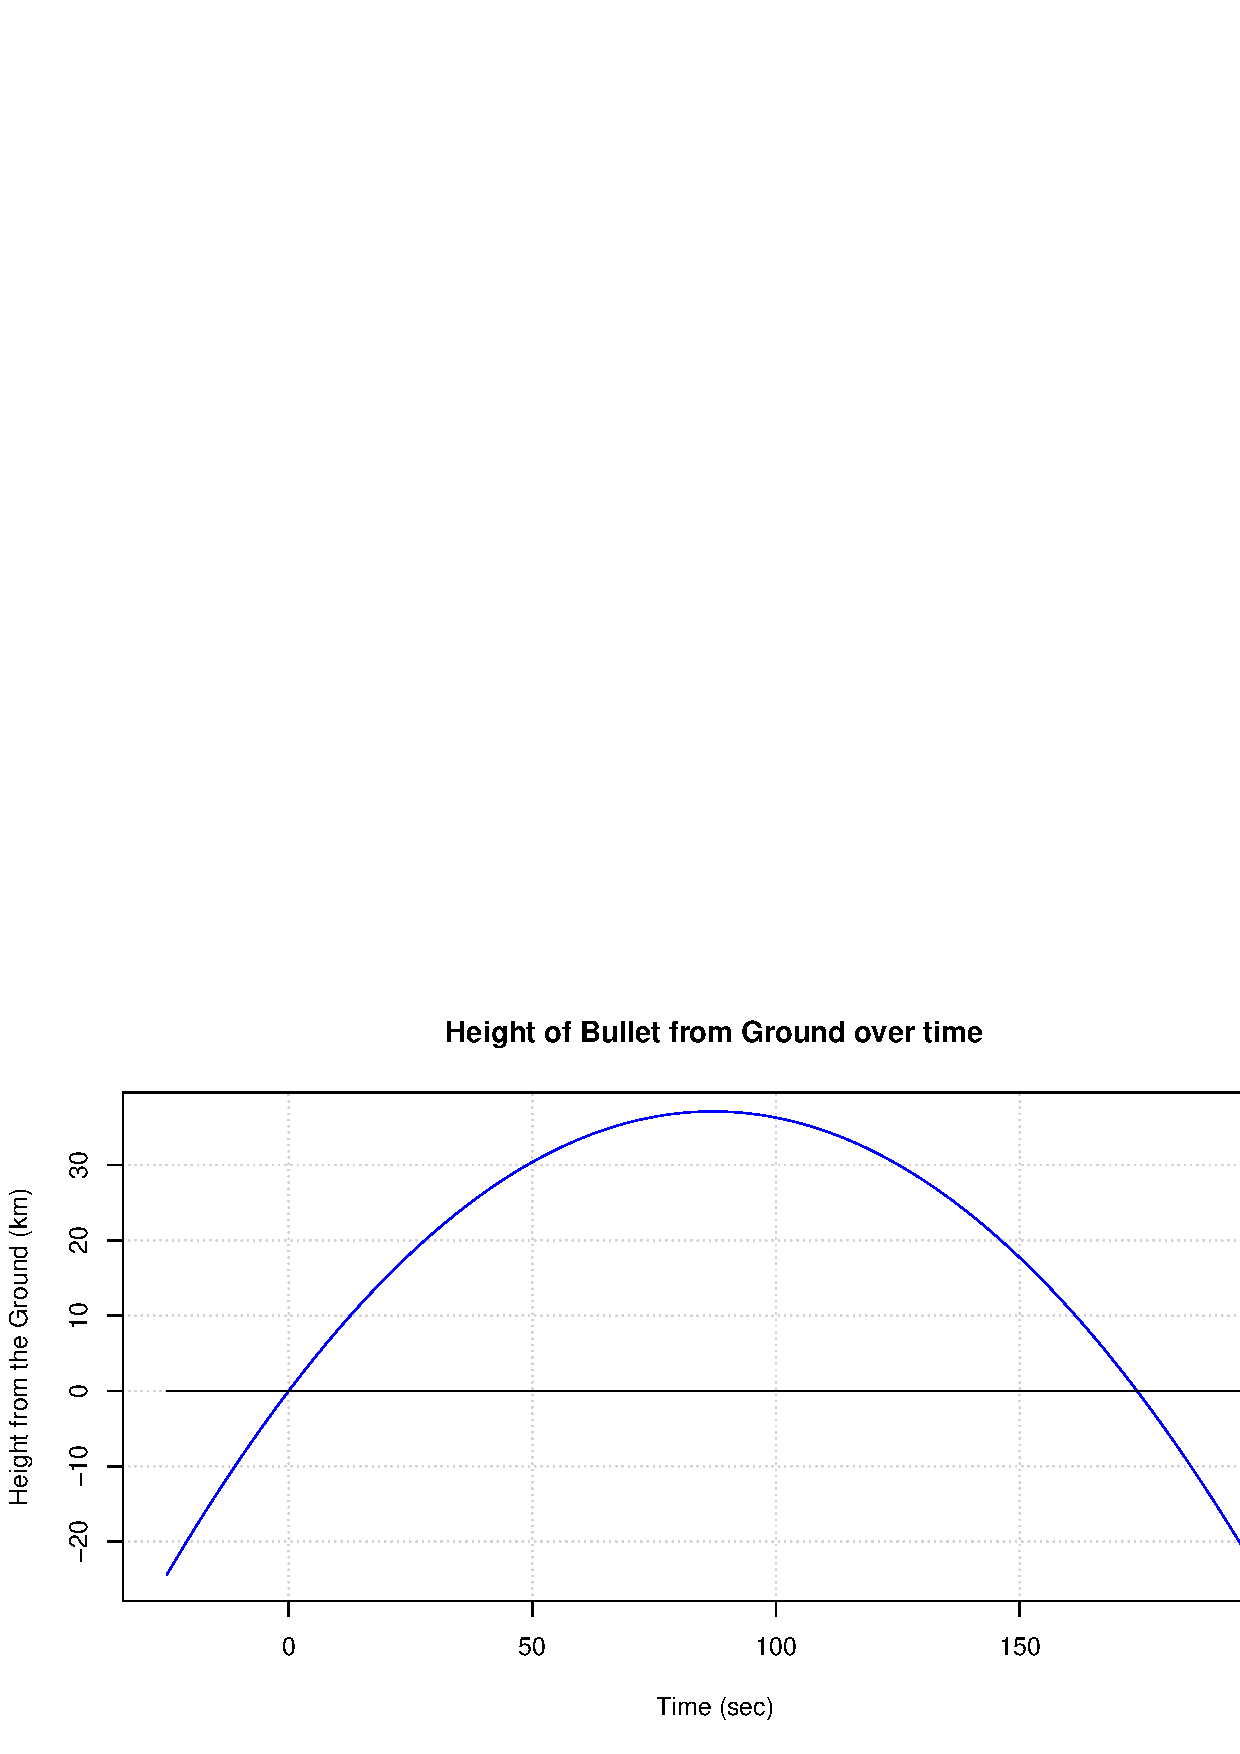
\includegraphics[width=.6\textwidth]{Prob1.png}
		\end{figure}
		\begin{enumerate}[label = (\alph*)]
			\item \[A_x = 5\cos\,130^\circ \approx -3.2139 \qqrarrow  A_y = 5\sin\,130^\circ \approx 3.8302 \]
			\item \[B_x = 4\cos\,210^\circ \approx -3.4641 \qqrarrow B_y = 4\sin\,210^\circ \approx -2.0000\]
			\item \[C_x = 5\cos\,(-45^\circ) \approx 3.5355  \qqrarrow C_y = 5\sin\,(-45^\circ) \approx -3.5355\]
		\end{enumerate}
	\end{problem}

	\begin{problem}{2}
		For each of the following vectors, determine its $x$-and $y$-components in terms of the magnitude of the vector, and either cosine or sine of the angle which is shown.  For example, if the angle shown is called $\phi$, then the answer will have either $\cos \phi$ or $\sin \phi$ in it.  The magnitude of the vector is indicated by a letter.  Any sine and cosine expressions should only have the given angle in them; for example, $\cos \phi$, not $\cos (90^\circ-\phi)$ or $\sin (90^\circ-\phi)$.
		\begin{figure}[h!]
			\centering
			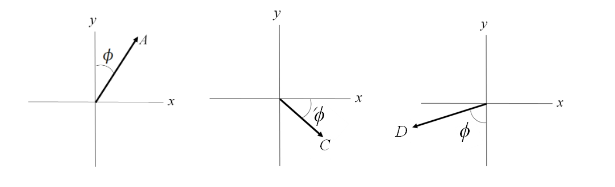
\includegraphics[width=.6\textwidth]{Prob2.png}
		\end{figure}
		\begin{enumerate}[label = (\alph*)]
			\item \[A_x = A\sin\phi \qqrarrow A_y = A\cos\phi\]
			\item \[C_x = C\cos\phi \qqrarrow C_y = -C\sin\phi\]
			\item \[D_x = -D\sin\phi \qqrarrow D_y = -D\cos\phi\]
		\end{enumerate}
		\begin{figure}[h!]
			\centering
			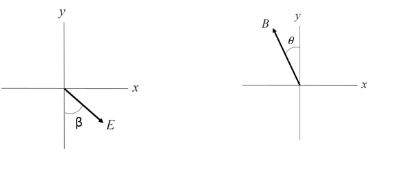
\includegraphics[width=.6\textwidth]{Prob2a.png}
		\end{figure}
		\begin{enumerate}[label = (\alph*)]
			\item[(d)] \[E_x = E\sin\beta \qqrarrow E_y = -E\cos\beta\]
			\item[(e)] \[B_x = -B\sin\theta \qqrarrow B_y = B\cos\theta\]
		\end{enumerate}
	\end{problem}

	\begin{problem}{3}
		A person undergoes two displacements: $\boldsymbol{\vec{A}}$, followed by $\boldsymbol{\vec{B}}$. The displacement vectors are shown in the diagram. Their magnitudes are:  $A=25$ m, $B=15$ m. (Their lengths are not drawn to scale in the diagram.) The purpose of this problem is to determine the magnitude and direction of the overall displacement vector for the whole trip (which is the vector sum $\boldsymbol{\vec{A}}$+$\boldsymbol{\vec{B}}$).  Follow the steps below. Give all answers to 2 decimal places.
		\begin{figure}[h!]
			\centering
			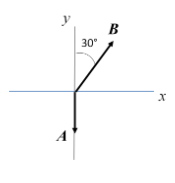
\includegraphics[width=.3\textwidth]{Prob3.png}
		\end{figure}
		\begin{enumerate}[label = (\alph*)]
			\item  Calculate the $x$-component and the $y$-component of $\boldsymbol{\vec{A}}$:
			\[A_x = 0 \qqrarrow A_y = -25\]
			\item  Calculate the $x$-component and the $y$-component of $\boldsymbol{\vec{B}}$:
			\[B_x = 15\sin\,30^\circ = 7.5 \qqrarrow B_y = 15\cos\,30^\circ = 7.5\sqrt{3}\]
			\item  Calculate the $x$-component and the $y$-component of the person’s overall displacement vector::
			\[A_x + B_x = 7.5 \qqrarrow A_y + B_y = -25 + 7.5\sqrt{3}\]
			\item Calculate the magnitude of the overall displacement vector.
			\[|A + B| = 14.1591\]
			\item Use your diagram in (d), and trigonometry, to determine the direction of the overall displacement vector, expressed as an angle measured counterclockwise from the positive x-axis.
			\[\theta = -58.0152\]
			\item \[\text{How Far } = 14.1591 \qqrarrow \text{Direction } = 58.0152\]
		\end{enumerate}
		
	\end{problem}


\end{document}
